\documentclass[12pt]{article}
\usepackage[margin=1in]{geometry}
\usepackage{graphicx}
\usepackage{booktabs}
\usepackage{amsmath}

\title{The Effect of Paid Search Advertising on Revenue: \\
A Replication of the eBay Natural Experiment}
\author{Your Name}
\date{\today}

\begin{document}
\maketitle

\section{Introduction}
This paper examines the causal effect of paid search advertising on eBay’s revenue, replicating the natural experiment studied by Blake, Nosko, and Tadelis (2014). Measuring the returns to search engine marketing (SEM) is challenging because advertising exposure is correlated with consumer intent, and users who click on ads are often already likely to purchase. This creates an endogeneity problem that biases naïve estimates upward. To address this, the original study exploits a natural experiment in which eBay suspended paid search advertising in a subset of geographic markets. Using a difference-in-differences framework that compares treated and control markets before and after the intervention, this replication estimates the causal impact of paid search on revenue.

\section{Experimental Setting}
Blake, Nosko, and Tadelis (2014) conducted a large-scale field experiment in collaboration with eBay to measure the causal effect of paid search advertising. In this experiment, eBay stopped bidding on Google AdWords in 65 out of 210 designated market areas (DMAs) in the United States, which were assigned to the treatment group beginning on May 22, 2012. This treatment lasted for approximately eight weeks. The remaining DMAs served as the control group, where paid search advertising continued. In the data, this corresponds to \texttt{search\_stays\_on = 0} for treated markets and \texttt{search\_stays\_on = 1} for control markets.

Importantly, the experiment was not fully randomized. The largest DMAs, which account for a disproportionate share of eBay’s revenue, were excluded from the treatment group. As a result, treatment and control markets differ systematically in their baseline revenue levels, with control markets generally exhibiting higher average revenue. This imbalance makes a simple comparison of average outcomes between treated and control groups potentially misleading. To address this issue, the analysis relies on a difference-in-differences framework, which compares changes in revenue over time between the two groups. By focusing on pre- and post-treatment differences, this approach isolates the causal effect of turning off paid search advertising under the parallel trends assumption.

\section{Data and Figures}
The dataset consists of daily revenue observations for 210 designated market areas (DMAs) in the United States from April to July 2012. Key variables include the date, DMA identifier, an indicator for the treatment period, a group indicator denoting whether paid search advertising was turned off or remained on, and total daily revenue. This panel structure allows for comparison of revenue patterns across treatment and control groups before and after the intervention.

\begin{figure}[h]
\centering
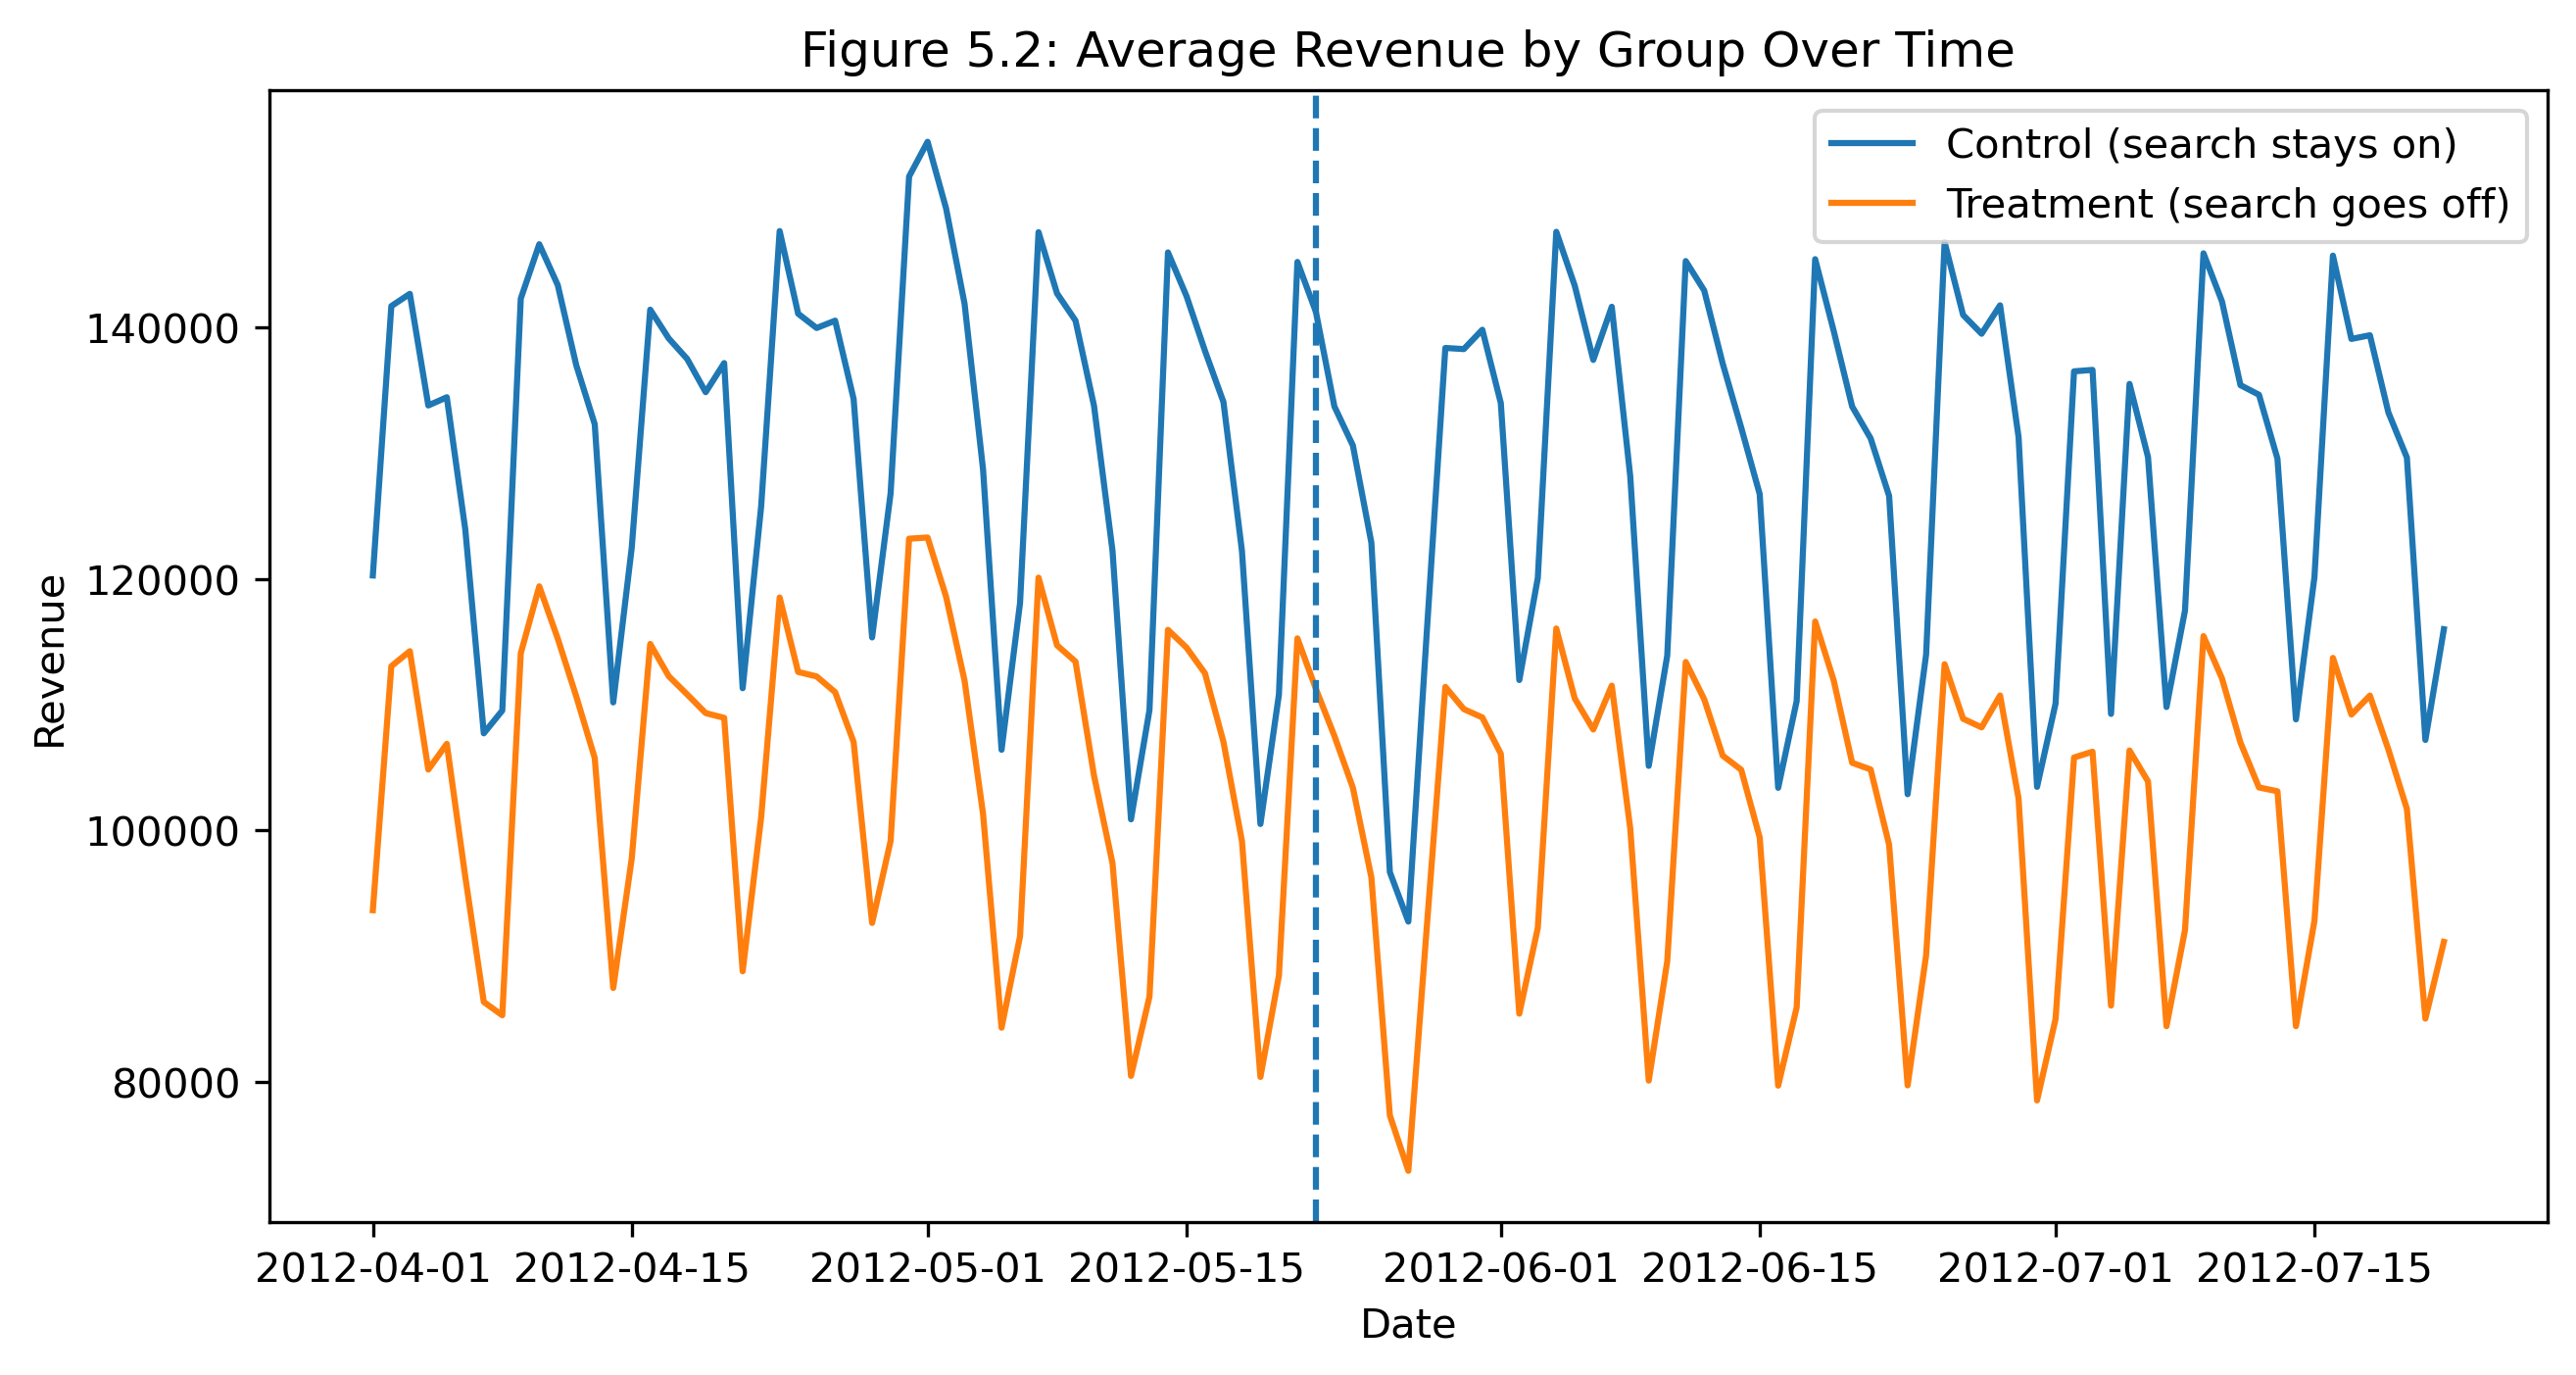
\includegraphics[width=0.85\textwidth]{../output/figures/figure_5_2.png}
\caption{Average revenue for treatment and control DMAs over time. The dashed line marks May 22, 2012, when SEM was turned off for the treatment group.}
\label{fig:revenue}
\end{figure}

Figure 5.2 plots average daily revenue over time for the control and treatment groups, with the vertical dashed line marking the start of the intervention. Prior to the intervention, both groups exhibit similar cyclical patterns, suggesting comparable trends over time. The control group consistently maintains a higher revenue level, reflecting baseline differences across markets. Following the intervention, the treatment group shows a slight and somewhat noisy decrease in revenue, though the magnitude of this change is small relative to the underlying seasonal variation. Overall, there is no clear visual evidence of a large divergence between the groups after the intervention.

\begin{figure}[h]
\centering
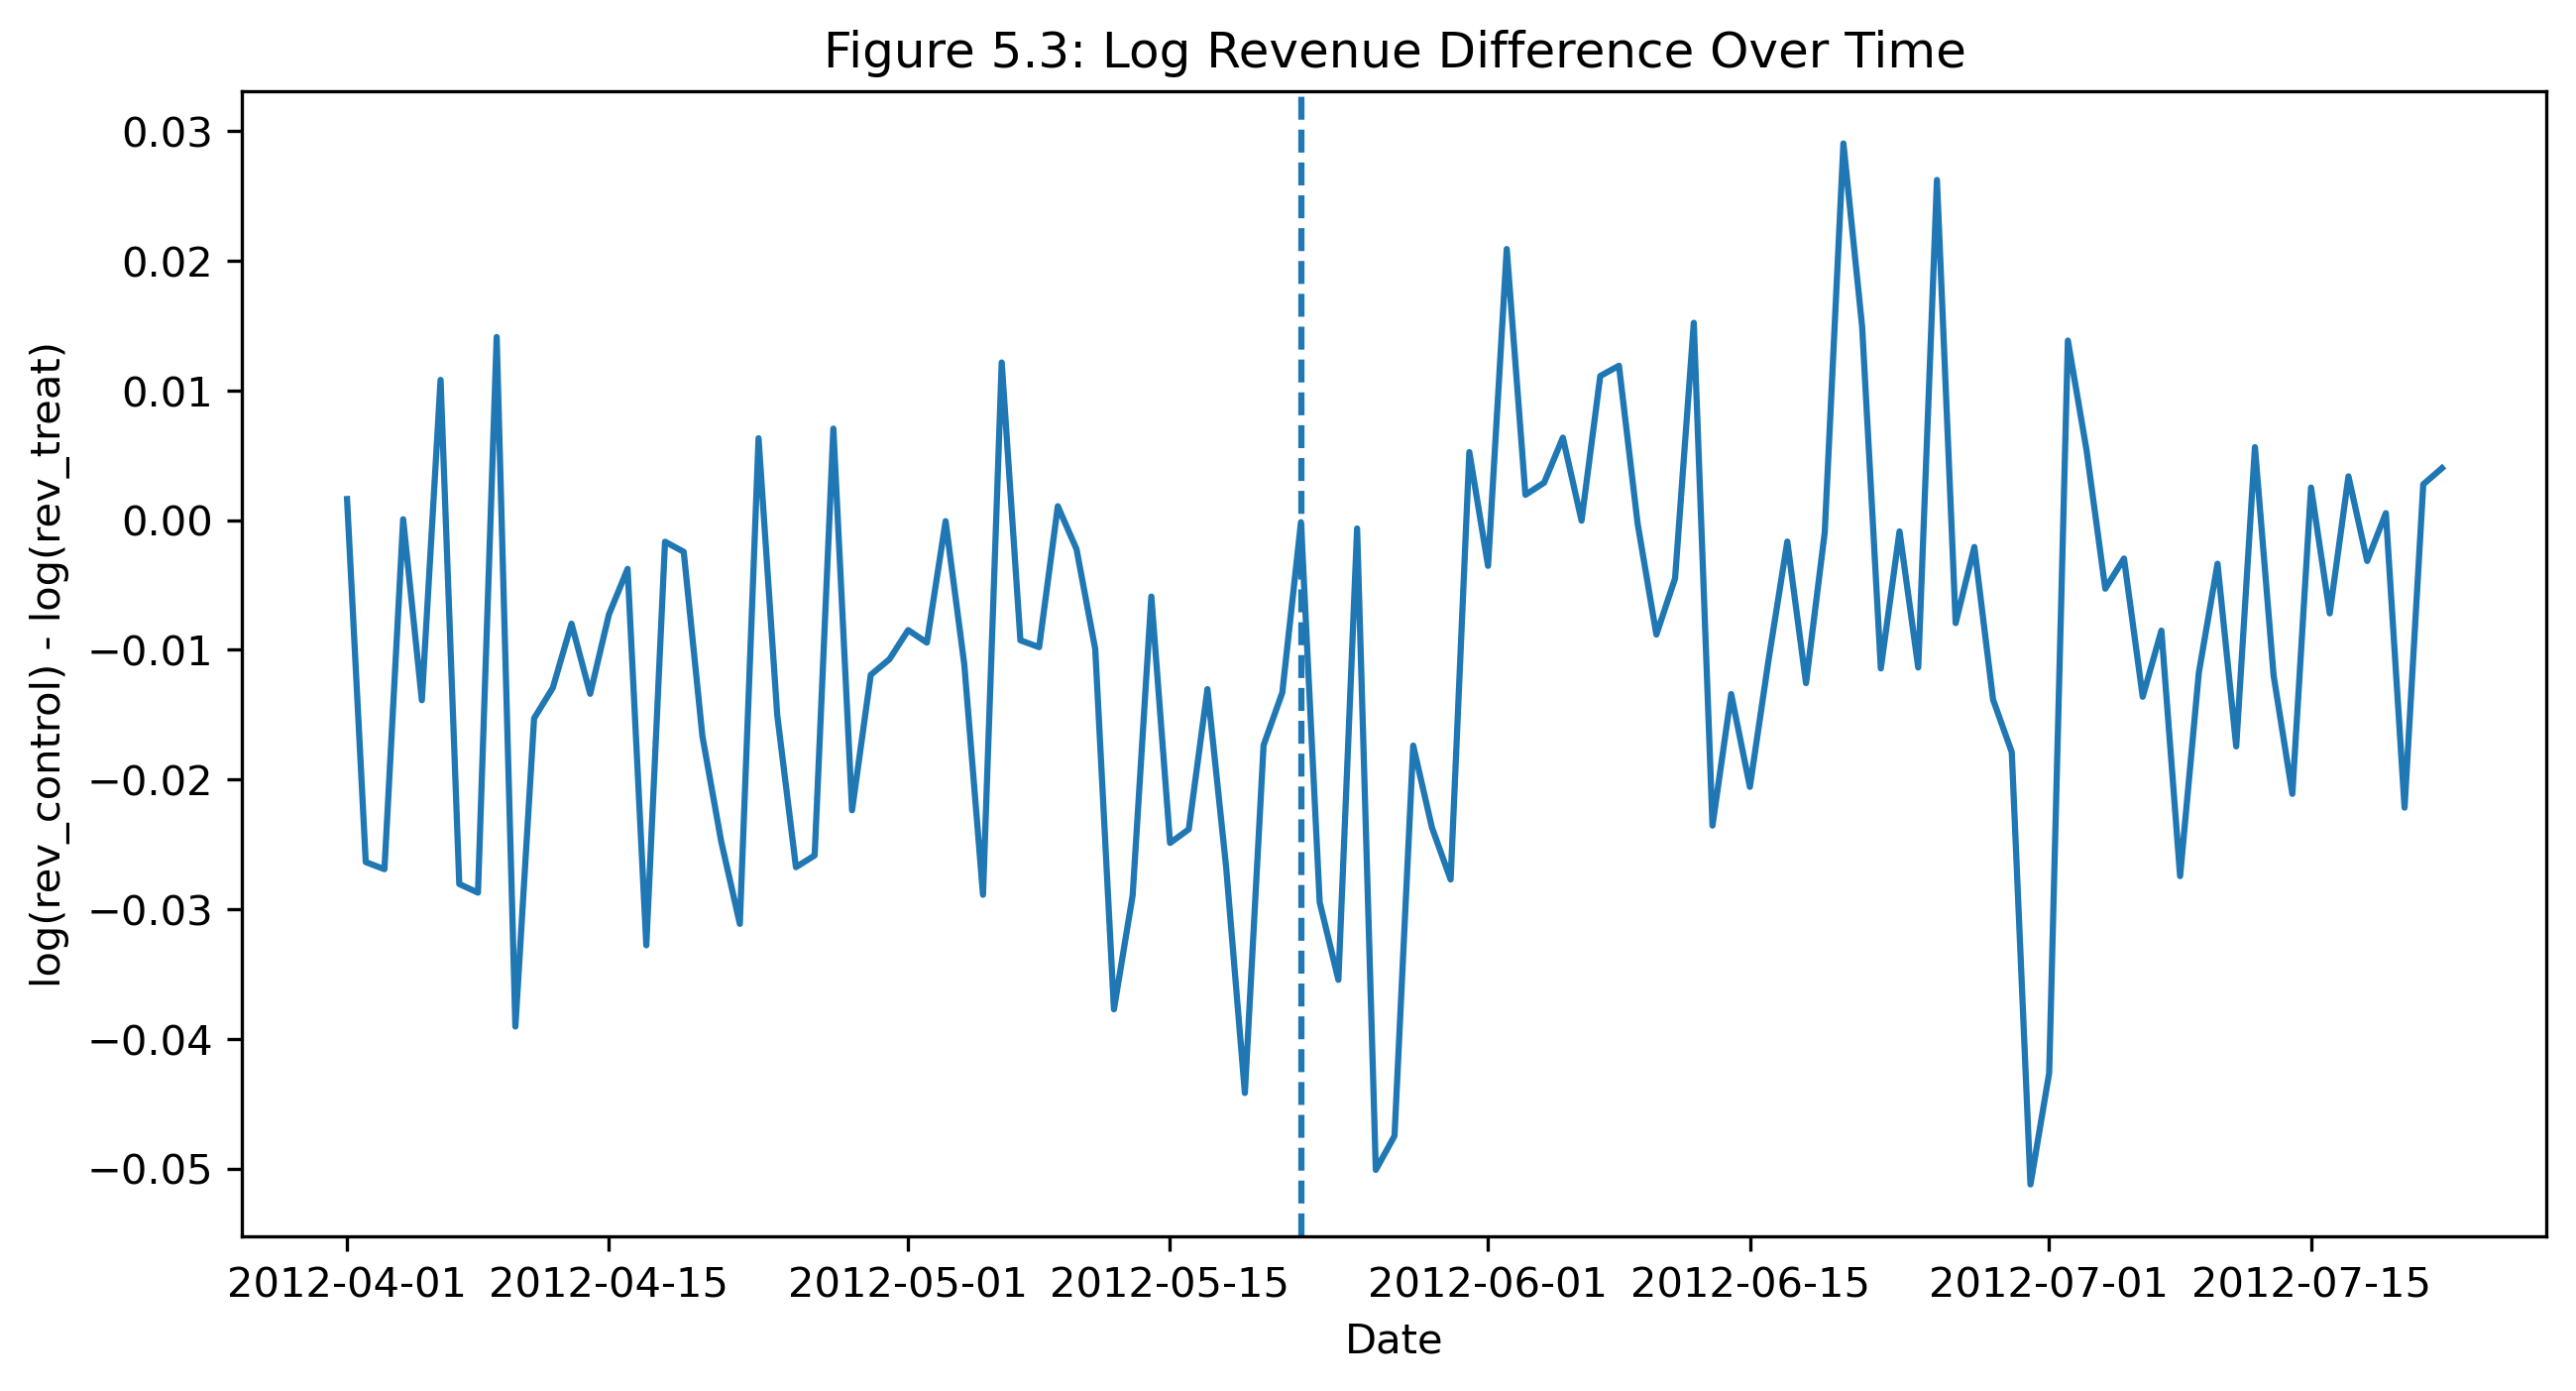
\includegraphics[width=0.85\textwidth]{../output/figures/figure_5_3.png}
\caption{Log-scale average revenue difference between control and treatment groups over time. The gap appears to increase after May 22.}
\label{fig:logdiff}
\end{figure}

Figure 5.3 plots the log difference in average revenue between the control and treatment groups over time. Prior to the intervention, the log difference fluctuates around a relatively stable level, suggesting that the gap between the two groups is approximately constant in the pre-treatment period. This stability supports the parallel trends assumption underlying the difference-in-differences approach. Following the intervention, the log difference appears to increase slightly, indicating a modest widening of the gap between control and treatment groups. However, this change is small and noisy, making it difficult to draw strong conclusions based on visual inspection alone. This pattern motivates the use of a formal difference-in-differences estimation to quantify the effect of paid search advertising.

\section{Results}
\input{../output/tables/did_table.tex}

Table \ref{tab:did} reports the difference-in-differences estimate of the effect of paid search advertising on revenue. The estimated treatment effect is $\hat{\gamma} = -0.0066$ in log terms, which corresponds to an approximate 0.66\% decrease in revenue when paid search advertising is turned off. Converting this estimate to levels yields $\exp(\hat{\gamma}) = 0.9934$, indicating that treated markets experienced slightly lower revenue relative to control markets. However, the 95\% confidence interval for the log estimate, $[-0.0175, \; 0.0043]$, includes zero, implying that the effect is not statistically significant at the 5\% level. Similarly, the confidence interval in levels includes one, reinforcing the conclusion that the effect is indistinguishable from zero.

Overall, the results suggest that turning off paid search advertising has a small and statistically insignificant impact on eBay’s revenue. This finding is consistent with Blake et al. (2014) and supports the interpretation that for a well-known brand, most users would have reached the website through alternative channels such as organic search even in the absence of paid advertising.

\section{Conclusion}
This paper replicates the difference-in-differences analysis of Blake et al. (2014) to estimate the causal effect of paid search advertising on eBay’s revenue. The results indicate a small and statistically insignificant effect, suggesting that turning off paid search advertising leads to little to no change in revenue. This finding is consistent with the original study and highlights the importance of distinguishing between correlation and causation when evaluating advertising effectiveness.

Several limitations should be noted. The data used in this analysis are scaled and do not reflect actual revenue levels, the treatment assignment was not fully randomized, and the empirical approach relies on a simple difference-in-differences framework without additional controls. Despite these limitations, the results provide evidence that for a well-known brand like eBay, paid search advertising may offer limited incremental value. More broadly, this underscores the importance of using experimental or quasi-experimental methods when measuring the return on marketing investments.

\begin{thebibliography}{9}
\bibitem{blake2014}
Blake, T., C. Nosko, and S. Tadelis (2014).
``Consumer Heterogeneity and Paid Search Effectiveness: A Large-Scale Field Experiment.''
\textit{Econometrica}, 83(1): 155--174.

\bibitem{taddy2019}
Taddy, M. (2019).
\textit{Business Data Science}. McGraw-Hill, Chapter 5.
\end{thebibliography}

\end{document}
